\chapter{Introduction}

Anthropogenic climate change is a real problem and has been stated as ``a threat to human well-being and the health of the planet" by the Intergovernmental Panel on Climate Change (IPCC) \cite{ipcc_2022}. The driving force behind climate change has to do with the emissions of green house gases into the atmosphere. According to data from the United States Environmental Protection Agency, carbon dioxide (CO$_2$) accounts for nearly three quarters of those greenhouse emissions \cite{epa_2019}. A breakdown of emissions by sector can be seen in figure \ref{fig:green_house_gas_emissions}.

\begin{figure}[h!]
	\centering
	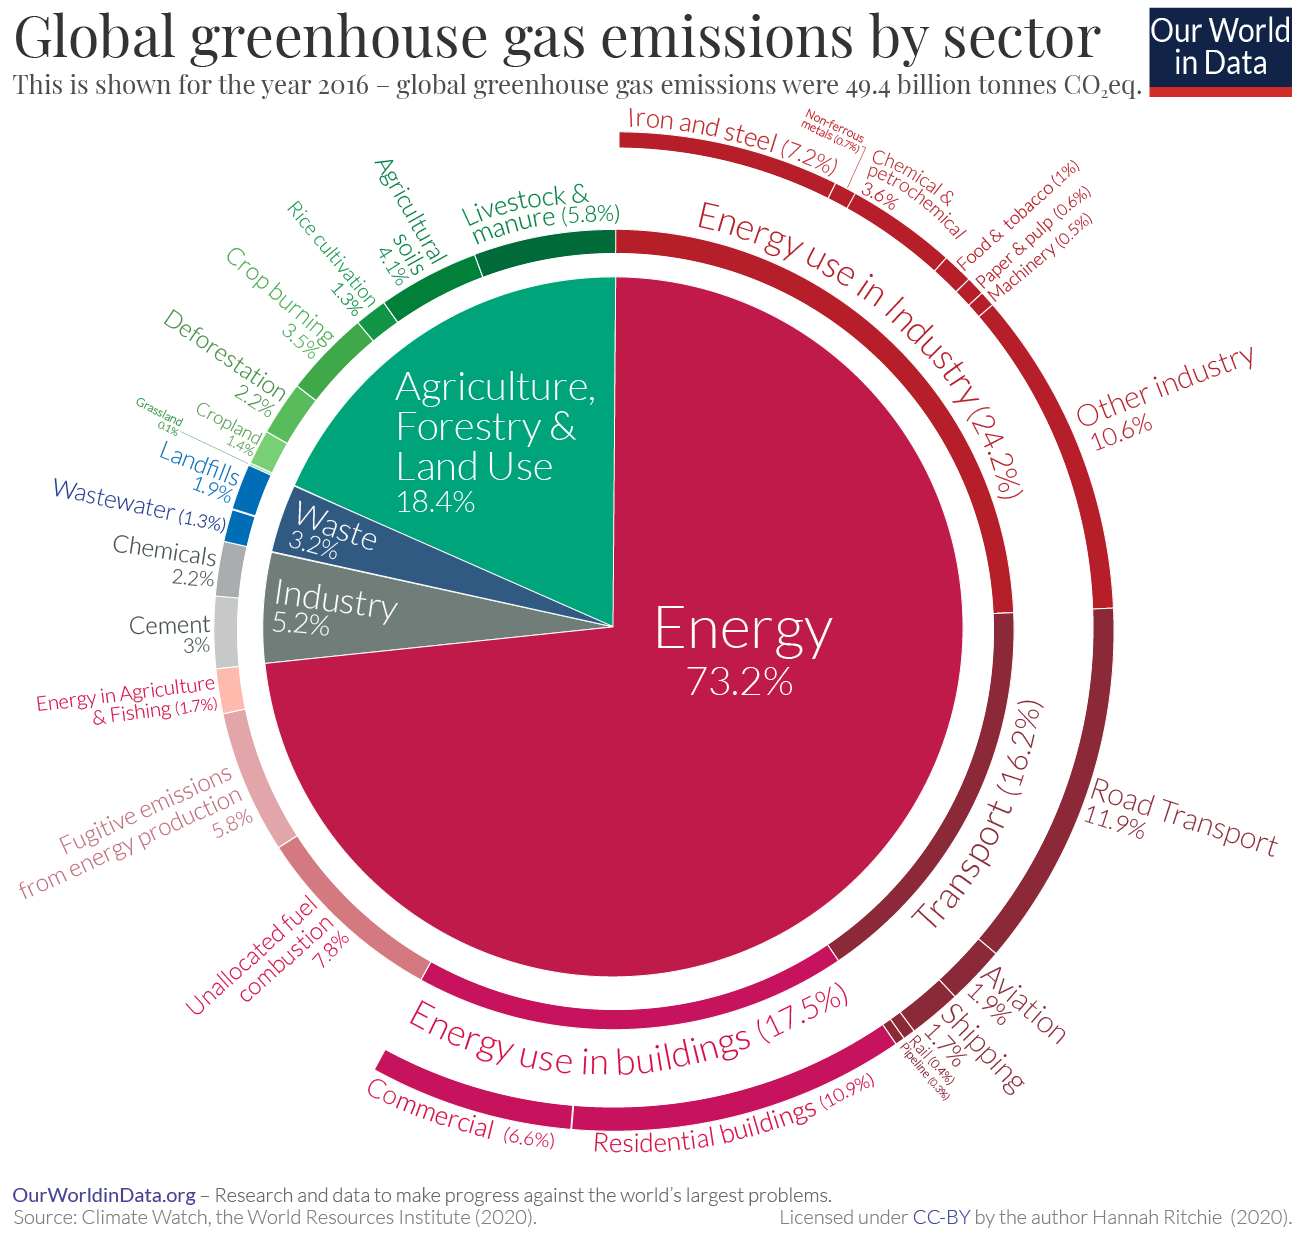
\includegraphics[width=0.7\linewidth]{chapter_1/figures/emissions.png}
	\caption{Global greenhouse gas emissions by sector \cite{ritchie_roser_2020}.}
	\label{fig:green_house_gas_emissions}
\end{figure} 

As seen in figure \ref{fig:green_house_gas_emissions}, global greenhouse emissions come from a variety of sources and processes. Hence, simply focusing efforts in areas such as transport or electricity generation is insufficient. Eliminating our dependance on fossil fuels by switching to renewables or driving electric cars is a start, but in order to achieve net-zero emissions, there needs to be innovations across various other sectors. Currently, there is no one solution to  climate change.

\section{Motivation}

Now, supposing that we have successfully decarbonised the economy, there will always be industrial processes that produce CO$_2$ as a byproduct. The quintessential example of this is the manufacturing of concrete, where the CO$_2$ is released from a chemical process due to the conversion of calcium carbonate (CaCO$_3$) to calcium oxide (CaO), rather than through combustion. As such it would be useful to capture this CO$_2$ and potentially reuse it in other manufacturing processes. 

There have many different approaches in the literature, with recent examples including generating synthetic fuels using electrochemical CO$_2$ recycling \cite{ross_et_al_2019} and using algae to convert CO$_2$ into carbon fibre \cite{arnold_et_al_2018}. This report will specifically focus on the area of carbon conversion via CO$_2$ splitting; specifically, plasma-assisted CO$_2$ splitting.


\section{Novelty}

Plasma-assisted CO$_2$ splitting is a relatively new technology that could be used for the process carbon conversion. In order to generate and sustain this plasma, inert feed gases (typically argon or helium) are oftentimes required. While the use of these feed gases are perfectly viable in a research laboratory setting, when it comes to scaling the process to an industrial level, the costs associated become untenable.

The novelty with this project is to asses the viability of a plasma driven carbon utilisation process that recirculats the feed gas, reducing the cost associated with the use of inert gases. This would require a control system to maintain the pressure of the feed gas as there will inevitably be some losses. It would also require the filtration of any waste products produced from the CO$_2$ splitting process and subsequent chemical reactions.

The rest of this report is structured as follows. A introduction of plasma discharges can be found in chapter 2. Chapter 3 goes on to provide an overview of the CO$_2$ splitting process. Then, chapter 4 provides a description of the process to design and develop the plasma reactor used for this project, along with some basic tests using only Helium gas. CO$_2$ gas is then introduced to the plasma reactor in chapter 5, where the results from the CO$_2$ splitting process can be found. Chapter 6 goes on to describe the mechanism of waste filtration and feed gas recirculation. Finally, the results of this report are discussed in the conclusion.